\section{Dinamica interna}\label{sec:dinamica-interna}
Arrivati a questo punto è interessante studiare la dinamica interna di queste galassie, ossia come si muovono le stelle al loro interno. Si nota infatti che le galassie a spirale e quelle ellittiche hanno una dinamica interna molto differente:

\begin{itemize}
    \item \emph{Galassie a spirale:} sono "rotation supported", ossia le stelle si muovono su orbite circolari (o quasi) attorno al centro (in modo molto ordinato). Le misure di cinematica interna si esplicano nella realizzazione di una curva di rotazione, che descrive come la rotazione delle stelle varia con al distanza dal centro galattico.
    \item \emph{Galassie ellittiche:} sono “pressure supported”, ossia le stelle su muovono di moti randomici attorno al centro (moto non ordinato). Una misura di cinematica si traduce nella realizzazione di un profilo di dispersione di velocità. Infatti noi dobbiamo pensare che il sistema si muove con un moto di insieme (il cosidetto "bulk motion") verso di me o lontano da me, ma ciascuna stella ha proprio moto. La dispersione di velocità misura quanto la velocità delle singole stelle sono disperse attorno alla velocità media del bulk motion, anche detta velocità sistemica.
\end{itemize} 

\subsection{Curve di rotazione delle galassie a spirale}

\begin{figure}
    \centering
    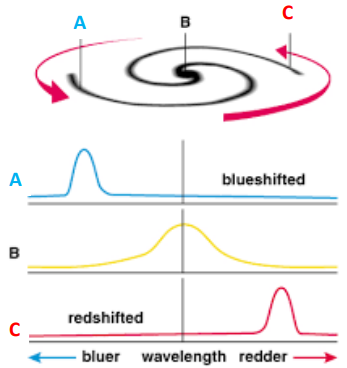
\includegraphics[width = 0.4 \textwidth]{immagini/effetto-doppler.png}
    \caption{La riga proveniente dal punto B (centro della galassia) ci dà la velocità sistemica, mentre le linee che provengono dai punti A e C ci dicono come si stanno muovendo i bracci della galassia: se si muovono verso di noi avranno emissione più spostata sul blu, mentre se si allontanano sul rosso.}
    \label{fig:effetto-doppler-galassie}
\end{figure}

Per analizzare la dinamica interna delle galassie a spirale ci serviamo di due strumenti principali:
\begin{itemize}
    \item Split spettroscopy: mettiamo una fenditura quando osserviamo una galassia, in modo da ricevere solo la luce caduta sulla fenditura: al centro della fenditura ci sarà la luce che proviene dal centro della galassia e la luce ai bordi della fenditura verrà invece dal bordo della galassia. Per costruire uno spettro a questo punto misuriamo una determinata riga spettrale, prima al centro e poi agli estremi della fenditura: quello che si ottiene è che la riga è centrata a lunghezze d’onda diverse per effetto Doppler. La riga della parte di galassia che si avvicina a noi è blue shifted e quella della parte di galassia che si allontana da noi è red shifter e attraverso una misura della differenza delle lunghezze d’onda delle parti estremali trovo la velocità di rotazione della galassia. La riga misurata al centro mi dice invece la velocità sistemica della galassia (tramite un confronto della lunghezza d’onda con quella di laboratorio), come viene riassunto in figura~\ref{fig:effetto-doppler-galassie}. La velocità di rotazione si misura utilizzando forti righe di emissione in banda otica e dalla riga 21cm in banda radio (viene da idrogeno neutro/gas freddo). 

    \item Integral Field spettroscopy: combina imaging (fotometria) e spettroscopia. Dopo aver ottenuto un’immagine della galassia, da ogni pixel del CCD otteniamo uno spettro. Abbiamo quindi un piano su cui si ha la luce che viene raccolta e una terza dimensione perché per ogni pixel c'è uno spettro. Questo ci permette di avere informazione sulla dinamica non solo sulla fenditura, come prima, ma su tutta l’area della galassia, quindi riusciamo ad ottenere delle mappe bidimensionali di rotazione. Mentre con la "split spettroscopy" abbiamo un valore di velocità per ogni distanza fissata dal centro, in questo modo otteniamo invece una mappa bidimensionale, quindi in ogni punto dell’area possiamo vedere quanto velocemente ruotano le stelle.
\end{itemize}

Le stelle in una galassia a spirale sono punti che ruotano attorno al centro, quindi  ci aspettiamo un potenziale kepleriano; la galassia però non è puntiforme. Dobbiamo quindi pensarla come a una sfera di gas e una stella che si muove in quella sfera. Al centro della galassia si ha rotazione nulla (infatti ci troviamo sull'asse di rotazione), poi ci sarà un andamento lineare della velocità fino a un certo punto, in cui possiamo ritornare al caso kepleriano, con un andamento riassunto in figura~\ref{fig:potenziale-galassie-a-spirale}.

\begin{figure}
    \centering
    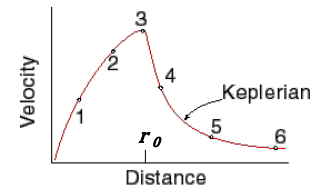
\includegraphics[width = 0.4 \textwidth]{immagini/potenziale-galassie-a-spirale.png}
    \caption{Andamento del potenziale nelle galassie a spirale.}
    \label{fig:potenziale-galassie-a-spirale}
\end{figure}

\begin{figure}
    \centering
    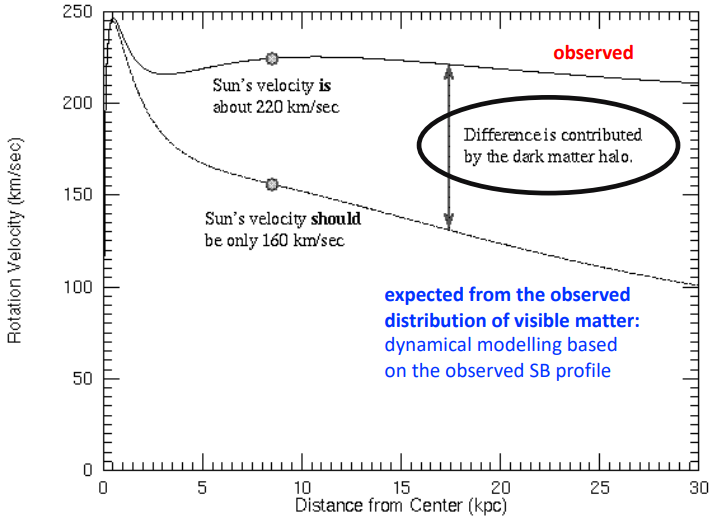
\includegraphics[width= 0.5\textwidth]{immagini/confronto-curve-di-rotazione.png}
    \caption{Confronto fra la curva di rotazione aspettata che segue un decadimento kepleriano e quella invece osservata, che non presenta questo decadimento ma piuttosto un plateu: questo fenomeno è spiegabile grazie alla materia oscura.}
    \label{fig:confronto-curve-di-rotazione}
\end{figure}

Dal punto 3 di figura~\ref{fig:potenziale-galassie-a-spirale}, siamo fuori dalla zona in cui c’è tanta materia, la densità è così bassa che posso approssimare la situazione come se fosse una massa puntiforme e quindi poi ci aspettiamo un andamento kepleriano Dal profilo di brillanza ci aspetteremo quindi un andamento dapprima con aumento lineare della velocità (fino a quando mi trovo abbastanza vicino alla galassia e più forza d'interazione c'è) e poi decrescita kepleriana. Guardando ai dati però non si osserva il “calo” kepleriano che ci aspetteremmo da come osserviamo la materia visibile. C'è una spiegazione a questo: l'unico modo per avere un andamento di questo tipo è infatti avere la presenza di una massa invisibile che continua ad essere presente anche quando ci aspettiamo che sia finiti la materia della galassia. Questa materia, che contribuisce alla buca di potenziale ma non è rilevabile attraverso emissione elettromagnetica, viene detta \emph{materia oscura}. In figura~\ref{fig:confronto-curve-di-rotazione} possiamo vedere le curve di rotazione relative alla nostra galassia, Via Lattea, con indicazione del Sole come sua stella. Come emerge dal confronto c'è una profonda discrepanza fra il comportamento aspettato e quello invece osservato, e questo è spiegabile solo ammettendo la presenza di questo alone di materia oscura che circonda anche la nostra galassia (addirittura si stima che la nostra galassia sia fatta al 75\% di materia oscura).

\subsection{Dispersione delle velocità per galassie ellittiche}

\begin{figure}
    \centering
    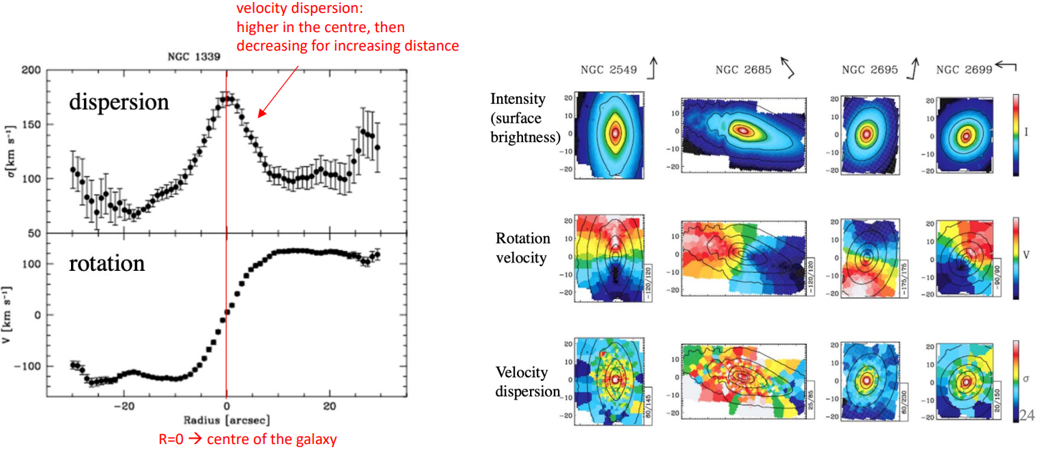
\includegraphics[width =0.7\textwidth]{immagini/spettroscopia-fessura-campo-integrale.png}
    \caption{Confronto fra i due tipi di spettroscopia: quella a fessura mi da una riga spettrale radiale, quella a campo integrale mi dà invece una mappa bidimensionale.}
    \label{fig:spettroscopia-fessura-campo-integrale}
\end{figure}

\begin{figure}
    \centering
    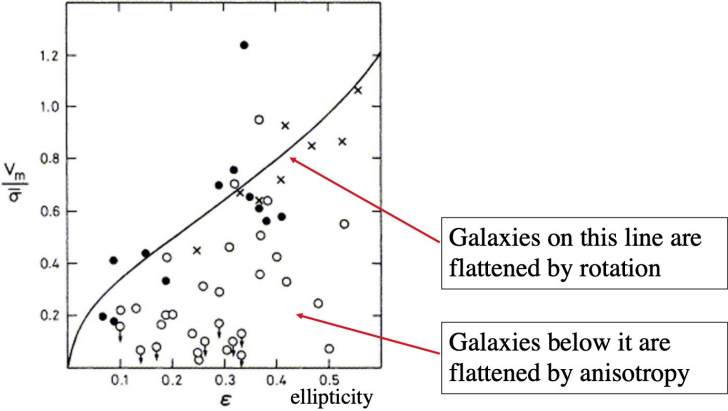
\includegraphics[width = 0.5\textwidth]{immagini/schiacciamento-galassie.png}
    \caption{La curva in figura divide le galassie che hanno velocità di rotazione sufficiente per causare in questo modo lo schiacciamento e quelle che invece sono schiacciate per anisotropia della dispersione di velocità. Possiamo vedere che la maggior parte delle galassie ellittiche (pallini) è schiacciata proprio per questo secondo motivo.}
    \label{fig:schiacciamento-galassie}
\end{figure}

Per quanto riguarda le galassie ellittiche, queste sono caratterizzate da una velocità media di movimento della galassia intera e poi in realtà ogni stella si muove random. Questi moti randomici hanno velocità distribuite con una distribuzione simile ad una gaussiana intorno alla velocità sistemica; si dice che le galassie ellittiche sono "pressure supported" perché più grande è la buca di potenziale e maggiore è la dispersione di velocità (quindi galassie più massicce hanno dispersione di velocità maggiore). Ci immaginiamo un allargamento della riga spettrale: ciascuna stella si muove con una velocità maggiore o minore rispetto alla velocità sistemica, quindi, avrà uno shift verso il blu o verso il rosso rispetto alla sistemica. Osserviamo una sovrapposizione di righe spettrali, alcune spostate verso il rosso e altre verso il blu; se la dispersione fosse zero avrei una distribuzione più stretta (gaussiana più stretta), quanto maggiore è la dispersione di velocità, tanto più larga è la distribuzione. A questo punto si misura l’allargamento al centro e a varie distanze dal centro e si ottiene un profilo di dispersione di velocità (sempre usando la spettroscopia a fessura). In modo alternativo si può procedere con la spettroscopia a campo integrale, in modo da ricavare una mappa bidimensionale di dispersione di velocità e non solo un profilo radiale. Un confronto tra i risultati ottenuti dai due tipi di spettroscopia è presentato in figura~\ref{fig:spettroscopia-fessura-campo-integrale}.

Un'altra caratteristica interessante delle galassie ellittiche è il loro schiacciamento: queste galassie infatti abbiamo detto che praticamentesi è detto infatti che non hanno una rotazione significativa, sorge quindi la domanda di come facciano ad essere schiacciate Questo fenomeno è in gran parte dovuta alla anisotropia orbitale (anisotropia della dispersione di velocità): questo significa che la dispersione di velocità non ha lo stesso valore in tutte le direzioni dello spazio. Se si ha una dispersione di velocità maggiore su un asse, avremo la galassia più allungata lungo tale direzione, ovvero la galassia risulta schiacciata nella direzione in cui si ha minore dispersione di velocità. La maggior parte delle ellittiche ha grande ellitticità pur con bassa velocità media di rotazione, come si può vedere in figura~\ref{fig:schiacciamento-galassie}.

\subsection{Materia oscura nelle galassie ellittiche}
A questo punto possiamo chiederci, se è presente un'evidenza di materia oscura anche nelle galassie ellittiche come c’è nelle galassie a spirale? La risposta è che per le galassie ellittiche è molto complicato osservare prove sperimentali per una serie di motivi:
\begin{itemize}
    \item Le ellittiche non sono rotanti e non posso costruire una curva di rotazione come nelle spirali, che ricordiamo nel caso delle spirali sono proprio queste curve che mettono in evidenza la presenza della materia oscura.
    \item Non conosciamo la struttura 3D (invece delle galassie a spirale sappiamo che sono "schiacciate", ossia a meno del bulge centrale le stelle nei bracci si trovano tutte sullo stesso piano) e l’unica informazione a disposizione è il profilo di brillanza superficiale.
    \item Non sappiamo la forma 3D della distribuzione anisotropa delle velocità, potrebbero esserci delle differenze significative a seconda della "profondità".
    \item Mentre nelle galassie a spirale il gas freddo (H neutro) ha grande estensione radiale e ci permette tramite l'effetto Doppler di misurare la curva di rotazione a grandi distante, nelle ellittiche non ci sono “tracciatori” di massa (o buca di potenziale) a grande distanza dal centro.
\end{itemize} 

\begin{figure}
    \centering
    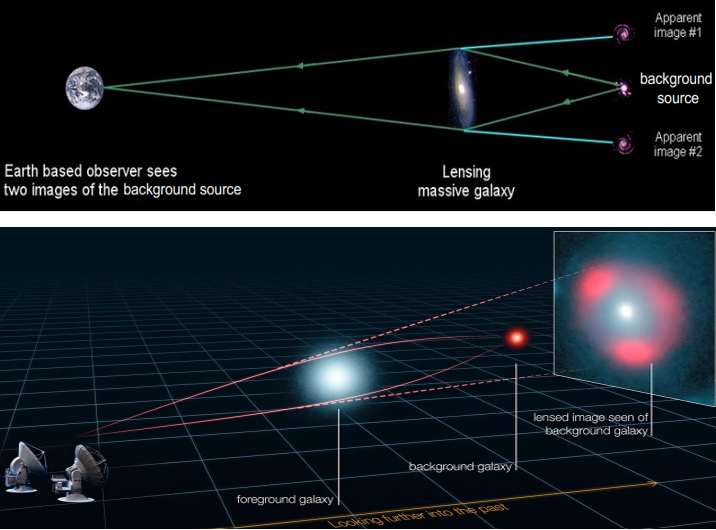
\includegraphics[width=0.6\textwidth]{immagini/gravitational-lensing.png}
    \caption{Il fenomeno del lensing gravitazionale può mostrarsi in due modi: possiamo osservare immagini multiple di una sorgente di background (sopra) o può comparire un anello attorno alla massa centrale (sotto).}
    \label{fig:gravitational-lensing}
\end{figure}

È molto difficile quindi ottenere dati sperimentali: un modo per stimare la massa è quello di usare il gas caldo diffuso, che emette in raggi X, presente in grande quantità nelle galassie ellittiche. Attraverso un’assunzione di equilibrio idrostatico, che è ragionevole per le ellittiche, possiamo stimare la massa della galassia (vedi capitolo ammassi di galassie).

Il metodo più utilizzato per stimare la massa di galassie ellittiche però è sfruttare il segnale che si ottiene dallo strong gravitational lensing. Si tratta fenomeno per cui la massa distorce lo spazio-tempo, di conseguenza i fotoni, anche se privi di massa, se nel tragitto tra sorgente e osservatore attraversano una sezione dello spazio-tempo distorta, deviano la loro traiettoria. A causa di questo, osservando un oggetto dalla Terra, compaiono immagini multiple della sorgente di background o, addirittura, può comparire un anello attorno alla massa centrale, detto anello di Einstein, anch'esso dovuto alla distorsione della luce da parte della galassia (come si può vedere in figura~\ref{fig:gravitational-lensing}). Attraverso questo effetto è possibile stimare la massa dell’oggetto responsabile dell’effetto; tipicamente si trova che la massa della lente (ossia della galassia ellittica interposta che fa da lente) è più grande della massa che posso stimare dalla luce dell’ellittica (usando il profilo di luce posso stimare la sua massa). In figura~\ref{fig:materia-oscura-ellittiche} si può vedere come, soprattutto a grandi raggi, sia necessaria quindi una correzione lineare all'andamento della densità di massa: per questo motivo si può interpretare la differenza fra la massa calcolata dal profilo di luce e quella calcolata dal lensing gravitazionale come la necessità di tenere conto di una componente addizionale di massa, composto da materia non barionica (oscura). Questo "alone", sembra quindi circondare anche le galassie ellittiche.

\begin{figure}
    \centering
    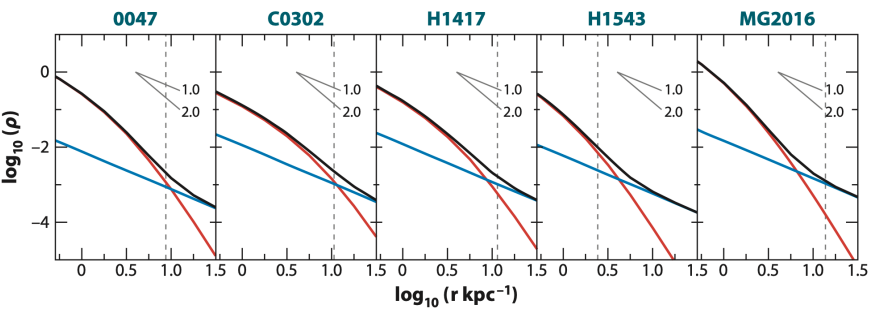
\includegraphics[width = 0.8 \textwidth]{immagini/materia-oscura-ellittiche.png}
    \caption{Densità di massa in funzione del raggio: si può vedere come per raggi grandi sia necessaria una correzione alla stima della massa, imputabile alla presenza di un alone di materia oscura anche attorno alle galassie ellittiche.}
    \label{fig:materia-oscura-ellittiche}
\end{figure}